% Created 2021-01-18 Mon 09:48
% Intended LaTeX compiler: pdflatex
\documentclass[presentation]{beamer}
\usepackage[utf8]{inputenc}
\usepackage[T1]{fontenc}
\usepackage{graphicx}
\usepackage{grffile}
\usepackage{longtable}
\usepackage{wrapfig}
\usepackage{rotating}
\usepackage[normalem]{ulem}
\usepackage{amsmath}
\usepackage{textcomp}
\usepackage{amssymb}
\usepackage{capt-of}
\usepackage{hyperref}
\usetheme{UoB}
\author{Mark Blyth}
\date{\textit{[2021-01-18 Mon]}}
\title{Discretisation: the beginning of the end?}
\hypersetup{
 pdfauthor={Mark Blyth},
 pdftitle={Discretisation: the beginning of the end?},
 pdfkeywords={},
 pdfsubject={},
 pdfcreator={Emacs 27.1 (Org mode 9.3)}, 
 pdflang={English}}
\begin{document}

\maketitle

\section{Background}
\label{sec:orgca5dbae}
\begin{frame}[label={sec:org3507513}]{Summary}
Fourier/Galerkin discretisation is inefficient for neuronal signals, so we need something better
\vfill
Last time:
\begin{itemize}
\item BSpline/Galerkin is numerically finicky
\item Orthogonal collocation cold be a suitable alternative method
\end{itemize}
\vfill
This time:
\begin{itemize}
\item Collocation progress
\item Progress on BSpline finickiness
\item Work plan for the year
\end{itemize}
\end{frame}

\section{Collocation}
\label{sec:org83a566a}
\begin{frame}[label={sec:org3fc5ef5}]{Collocation progress}
\begin{itemize}
\item Implemented `standard' orthogonal collocation
\begin{itemize}
\item Lagrange polynomial basis functions,  no control aspect
\end{itemize}
\end{itemize}
\vfill
\begin{itemize}
\item Reformulated for BSpline basis functions
\begin{itemize}
\item Using Lagrange polynomials gives a picewise-polynomial solution, much like splines
\item Key difference is spline basis includes smoothness requirements too, potentially useful for CBC
\item Spline knots define solution mesh, simplifying problem slightly
\item Numerically, both work nicely; can't rigorously say which one is better or worse
\end{itemize}
\end{itemize}
\vfill
\begin{itemize}
\item Finished during Christmas; yet to build into a control-based continuation
\end{itemize}
\end{frame}

\begin{frame}[label={sec:org65918f8}]{Collocation progress}
Numerical continuation of periodic orbits from a Hopf normal form
\begin{center}
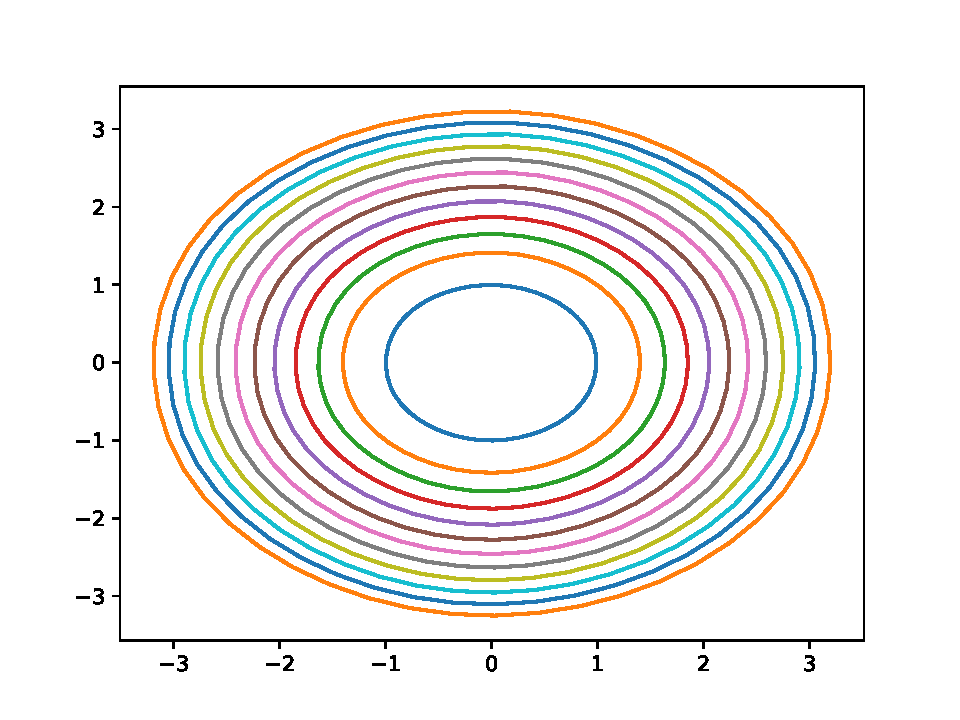
\includegraphics[width=.64\textwidth]{./collocation.pdf}
\end{center}
\end{frame}

\section{{\bfseries\sffamily TODO} More BSplines}
\label{sec:org67d9fd1}
\begin{frame}[label={sec:orgaebbf0b}]{Testing BSpline/Galerkin}
BSpline/Galerkin struggles on some parts of the solution curve; why? Tested\ldots{}
\begin{itemize}
\item Control gains: no major impact, within a sweetspot
\begin{itemize}
\item Big enough to stabilise UPOs, small enough to preserve numerical accuracy
\end{itemize}
\item Solvers: SciPy and my DIY Newton
\begin{itemize}
\item No difference, good to see; my solver is significantly slower
\item Suggests issues are from prediction/correction setup or existence-and-uniqueness, rather than Jacobian estimation
\end{itemize}
\item Stepsizes: has a big impact with Fourier/Galerkin
\begin{itemize}
\item Fourier/Galerkin can be made to fail in the same way as BSpline/Galerkin, when bad stepsizes are chosen
\item BSpline/Galerkin can't be made to work well when varying stepsizes
\item \emph{Maybe an adaptive stepsize is needed!}
\end{itemize}
\end{itemize}
\end{frame}

\begin{frame}[label={sec:org61a5437}]{Adaptive stepsize methods}
\begin{itemize}
\item Consider a prediction \(p(h)\), obtained for stepsize \(h\)
\item Newton correction \(c(h) = p(h) - J_f^{-1}|_{p(h)}f\left(p(h)\right)\)
\item Size of first step \(\delta(h)=\|J_{f}^{-1}|_{p(h)}f(p(h))\|\) estimates the error of the prediction
\item If \(\delta\) is too big, shorten the stepsize and try again
\item If \(\delta\) is too small, lengthen the stepsize for next time
\item Bonus: use an asymptotic expansion to choose the best stepsize
\end{itemize}
\end{frame}
\begin{frame}[label={sec:org4e43717}]{Adaptive stepsize methods}
\begin{itemize}
\item We can quantify the `speed of approach' with contraction rate \(\kappa\)
\[\kappa(h) := \frac{\|\text{second Newton step}\|}{\|\text{first Newton step}\|}\]
\item By asymptotic expansion, \(\kappa(h) = \varkappa h^2 + \mathcal{O}(h^3)\)
\end{itemize}
\vfill
Strategy:
\begin{itemize}
\item Choose target contraction rate
\item After each step, estimate the stepsize \(h=\sqrt{\frac{\kappa}{\varkappa}}\) that would have given our contraction rate
\item Use that, stepsize from \(\delta\) asymptotic expansion, and current stepsize to choose next stepsize
\end{itemize}
\end{frame}

\begin{frame}[label={sec:orgcafad04}]{Adaptive stepsize results}
\begin{itemize}
\item Monitoring contraction rate, and size of the first Newton correction
\item This gives a lot of extra hyperparameters: min, max stepsize; initial stepsize; nominal contraction rate and predictor error
\begin{itemize}
\item Getting results means choosing sensible values for all of these, which isn't easy!
\end{itemize}
\item Can't use the adaptive method with a pre-rolled solver; Newton Jacobian estimation is painfully slow; takes a long time to test hyperparameters
\begin{itemize}
\item Broyden update is the way to go
\end{itemize}
\end{itemize}
\vfill
No results so far; Newton solver diverges at first fold bifurcation, with or without adaptive stepsizes
\end{frame}

\begin{frame}[label={sec:org7a91f97}]{Solver divergence}
Issue: Newton solver diverges at first fold; doesn't happen with Fourier discretisation
\begin{itemize}
\item Wasn't previously an issue as I'd run only 1 Newton step
\begin{itemize}
\item Interesting that it does happen; probably a result of the control aspect
\end{itemize}
\item Convergence criteria: \(\|x_n - x_{n-1}\|<\mathrm{tol} ~~or f(x_n)<\mathrm{tol}\)
\begin{itemize}
\item With Fourier, \(x_n, f(x_n) \in \mathcal{O}(\mathrm{small})\)
\item With BSplines, \(x_n, f(x_n) \in \mathcal{O}(1)\)
\end{itemize}
\item Using the same tolerance implicitly applies looser convergence requirements to Fourier
\item Proposals:
\begin{itemize}
\item Use relative tolerances instead, eg. \(\sum_i\left(\frac{x^i_n-x^i_{n-1}} {x^i_n} \right)^2\)
\item Or, take the best solution from the first \(n\) iterations
\end{itemize}
\end{itemize}
\end{frame}

\section{Current work-plan}
\label{sec:org6ec74cb}
\begin{frame}[label={sec:org86bf620}]{Immediate plan}
Demonstrate how BSplines can be used for efficient CBC on slow-fast systems
\vfill
\begin{itemize}
\item Check that adaptive stepsizes \emph{do} make splines work
\item Switch Duffing for van der Pol oscillator
\item Implement an appropriate (CBC-inspired or numerical-inspired) phase constraint
\item Implement intelligent / adaptive BSpline knot selection
\begin{itemize}
\item BSpline knots generally need careful placement to be an efficient discretisor
\end{itemize}
\item If it all works, write it up!
\end{itemize}
\vfill
Perhaps focus more on how CBC can be used on slow/fast systems, and less on discretisation
\end{frame}

\begin{frame}[label={sec:org1ae1ca2}]{Mid-term plan}
Lots of other discretisations could work
\vfill
\begin{itemize}
\item Try collocation, wavelets, surrogate-based
\item Produce a recipe book of discretisation methods, suggesting which to use when
\item Develop an algo for the experiment to choose its best discretisor at each step?
\end{itemize}
\vfill
Covers similar research to the other proposed paper, challenge would be making it a unique contribution
\end{frame}

\section{Year work-plan + questions}
\label{sec:orgbf57850}
\begin{frame}[label={sec:org707089f}]{Long-term plan}
Automated neuronal identification and classification
\vfill
\begin{itemize}
\item Option 1: classify bursters from their fast subsystem bifurcations
\begin{itemize}
\item Approach 1: try to implement slow/fast analysis methods in a CBC framework
\item Approach 2: use feedback control to gather data for fitting cubic Lienard model; analyse fitted model to extract classification
\item Challenge: can't study each subsystem individually, on a real experiment
\end{itemize}
\item Option 2: couple CBC to model identification procedure, and fit a `generic' HH-model
\begin{itemize}
\item Can hopefully discover a cell's ion channels and their kinetics, without any a priori knowledge
\item Challenge: lots of different gating and conductance dynamics; a general model might be too general to accurately fit
\item Simplification: use voltage, current, dynamic clamp results as prior information; CBC then becomes an enhanced model fitting method
\end{itemize}
\end{itemize}
\end{frame}

\begin{frame}[label={sec:orgd46e714},plain]{Some questions}
\begin{itemize}
\item Are these ideas biologically useful?
\begin{itemize}
\item Burster classifications are interesting mathematically, but are they of biological significance?
\item Is a classification experiment of interest to experimenters, or is it more a mathematical toy?
\end{itemize}
\item Lots of interesting dynamics can appear in bursters and multi-timescale systems
\begin{itemize}
\item Mixed-mode oscillations, canards, torus canards, noise-induced bursting
\item Are these dynamics important biologically, or are they more mathematical curiosities?
\item Would slow-fast CBC be missing key biological dynamics by ignoring these behaviours?
\end{itemize}
\item Is slow/fast enough? Do we need additional (medium, or super-slow) timescales?
\begin{itemize}
\item Seen some papers using 3 timescales; are two-timescale models too simple to capture real dynamics?
\end{itemize}
\item Are burster classifications limited to single cells, or could the same methods reveal information about networks?
\end{itemize}
\end{frame}

\section{Next steps}
\label{sec:org9c3cf24}
\begin{frame}[label={sec:org99391ee}]{Next steps}
This wek: NODYCON slides and presentation; then\ldots{}
\vfill
\begin{itemize}
\item Try adaptive stepsizes to demonstrate splines success on Duffing oscillator
\end{itemize}
\vfill
\begin{itemize}
\item Generalise code to work on van der Pol oscillator
\begin{itemize}
\item Implement a phase constraint, and knot selection
\end{itemize}
\end{itemize}
\vfill
\begin{itemize}
\item Test it all out!
\end{itemize}
\end{frame}
\end{document}
